\chapter{Experiments}
\label{cha:exp}

In this chapter we will go through a set of experiments to showcase the result of taking different approaches toward file transfer techniques. Meanwhile we will try a number of data distribution methods to see how they fit into our scenarios.

\section{Distributed Hash Tables}
Distributed Hash Tables (DHT) known best for their application to build torrent tracking software, let us to have a key/value store and distributed it in a decentralized way amount a network of peers.

MORE INFO HERE ON DHT, KAMEDLIA PAPER and IMPLEMENTATIONS

In our case to keep track of the available data on the network of collaborating peers, we can use a DHT table. Everytime an instance wants to find a dataset it should query the network of peers using one of the existing wrappers and implementations.

\section{Test Results}
Our tests show that even though DHT is fault-tolerant and reliable for file distribution, it is not adequete for our realtime requirement to find our required data. In one test we ran two peers, one on an Internet host and another one on local host. Here are the client and server codes:

\begin{python}
from twisted.application import service, internet
from twisted.python.log import ILogObserver

import sys, os
sys.path.append(os.path.dirname(__file__))
from kademlia.network import Server
from kademlia import log

application = service.Application("kademlia")
application.setComponent(ILogObserver, 
	log.FileLogObserver(sys.stdout, log.INFO).emit)

if os.path.isfile('cache.pickle'):
    kserver = Server.loadState('cache.pickle')
else:
    kserver = Server()
    kserver.bootstrap([("178.62.215.131", 8468)])
kserver.saveStateRegularly('cache.pickle', 10)

server = internet.UDPServer(8468, kserver.protocol)
server.setServiceParent(application)


# Exposing Kademlia get/set API
from txzmq import ZmqEndpoint, ZmqFactory, ZmqREPConnection,
 ZmqREQConnection

zf = ZmqFactory()
e = ZmqEndpoint("bind", "tcp://127.0.0.1:40001")

s = ZmqREPConnection(zf, e)

def getDone(result, msgId, s):
    print "Key result:", result
    s.reply(msgId, str(result))

def doGetSet(msgId, *args):
    print("Inside doPrint")
    print msgId, args

    if args[0] == "set:":
        kserver.set(args[1], args[2])
        s.reply(msgId, 'OK')
    elif args[0] == "get:":
        print args[1]
        kserver.get(args[1]).addCallback(getDone, msgId, s)
    else:
        s.reply(msgId, "Err")

s.gotMessage = doGetSet
\end{python}

In the above example we have used \textit{twisted} networking library\cite{TwistedMatrix} and one python implementation\cite{KademliaImpl} of \textit{Kademlia} DHT algorithm\cite{KademliaPaper}. This will start a p2p network and will try to bootstrap it with another peer on the give IP address. Thereafter it will open another endpoint to expose a simple \textit{get/set} method for the rest of application for communicating with the network.

HERE DESCRIBE ABOUT DHT IMPLEMENTATION AND TWISTED NETWORKING LIBRARY. ***MOST IMPORTANT*** ABOUT REPLICATION OF DATA, IS THERE ANY REPLICATION? WHAT IF A NETWORK NODE FAILS? ***RCP OVER UDP AND WORK THROUGH FIREWALLS***

The next part is a few lines of code to communicate with this network:

\begin{python}
#
# Request-reply client in Python
# Connects REQ socket to tcp://localhost:5559
# Sends "Hello" to server, expects "World" back
#
import zmq

# Prepare our context and sockets
context = zmq.Context()
socket = context.socket(zmq.REQ)
socket.connect("tcp://localhost:40001")

# Set request
socket.send(b"set:", zmq.SNDMORE)
socket.send(b"the key", zmq.SNDMORE)
socket.send(b"the value")
print socket.recv()

# Get request
socket.send(b"get:", zmq.SNDMORE)
socket.send(b"the key")
print socket.recv()

# Invalid get
socket.send(b"get:", zmq.SNDMORE)
socket.send(b"not existing")
print socket.recv()
\end{python}

This simple client will try to connect to the previously opened port and send get/set messages.

\subsection{The Problem}
Configuring this p2p network is a little tricky. The network should work correctly even if nodes enter and leave the network. During our tests in development environment we observed some problems with initializing the network, but while the network was initialized leaving and entering the network had no effect on the results.

\subsubsection{Reliability}
Having the number of nodes increased up to 3 the reliability shows up again. When we set a value for a key in one node we can not guarantee that getting the value for that key on other nodes will return the updated one. With a number of tests I can confirm that two nodes which are bootstrapped with the same third node does not provide the accurate result everytime and it is not clear for me why this happens. See figure~\ref{fig:threepeers} on page ~\pageref{fig:threepeers}.

After running more tests, we figured out that the possible source of the above mentioned problems was the confusion in using \textit{binary} and \textit{string} in python, so it was an error in our side.

\begin{figure}
\centering
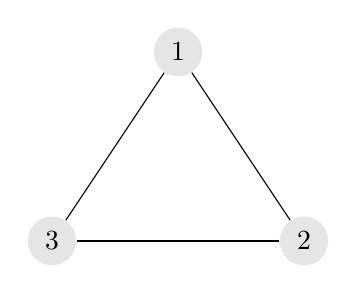
\begin{tikzpicture}
  [scale=.8,auto=left,every node/.style={circle,fill=gray!20}]
  \node (n1) at (5,5) {1};
  \node (n2) at (7,2)  {2};
  \node (n3) at (3,2)  {3};

  \foreach \from/\to in {n1/n2,n1/n3,n2/n3}
    \draw (\from) -- (\to);
\end{tikzpicture}
\caption{A network of three peers}
\label{fig:threepeers}
\end{figure}


\subsubsection{Firewall Problems}
In a test having one process running on a server in Internet and outside of the local network and having two different processes running on one laptop but on different ports it is observed that the changes (sets) in the internet does not replicate to the local processes but the changes from local processes are being replicated to the other process.

\subsection{conclusion}
Having a network between local and internet processes in the above mentioned method is not reliable. Repeating the tests with only local processes which are bootstrapping to one of them and running the setter/getter methods showed that even in this scenario it is not reliable and one can not guarantee that the desired value will be returned.


